% !TeX program = pdfLaTeX
\documentclass[smallextended]{svjour3}       % onecolumn (second format)
%\documentclass[twocolumn]{svjour3}          % twocolumn
%
\smartqed  % flush right qed marks, e.g. at end of proof
%
\usepackage{amsmath}
\usepackage{graphicx}
\usepackage[utf8]{inputenc}

\usepackage[hyphens]{url} % not crucial - just used below for the URL
\usepackage{hyperref}
\providecommand{\tightlist}{%
  \setlength{\itemsep}{0pt}\setlength{\parskip}{0pt}}

%
% \usepackage{mathptmx}      % use Times fonts if available on your TeX system
%
% insert here the call for the packages your document requires
%\usepackage{latexsym}
% etc.
%
% please place your own definitions here and don't use \def but
% \newcommand{}{}
%
% Insert the name of "your journal" with
% \journalname{myjournal}
%

%% load any required packages here
\usepackage{caption}
\usepackage{tabularx}
\usepackage{multirow}
\usepackage{placeins}
\usepackage{float}
\usepackage[modulo]{lineno}
\usepackage{xcolor}
\usepackage[none]{hyphenat}


% Pandoc citation processing


\begin{document}

\title{Open-source tools in R for landscape ecology }



\author{  Maximillian H.K. Hesselbarth \and  Jakub Nowosad \and  Johannes Signer \and  Laura J. Graham \and  }


\institute{
        Maximillian H.K. Hesselbarth \at
     a) Department of Ecosystem Modelling, University of Goettingen, Buesgenweg 4, 37077 Goettingen, Germany b) Department of Ecology and Evolutionary Biology, University of Michigan, Ann Arbor, MI, 48109, USA \\
     \email{\href{mailto:mhk.hesselbarth@gmail.com}{\nolinkurl{mhk.hesselbarth@gmail.com}}}  %  \\
%             \emph{Present address:} of F. Author  %  if needed
    \and
        Jakub Nowosad \at
     Institute of Geoecology and Geoinformation, Adam Mickiewicz University, Krygowskiego 10, 61-680 Poznan, Poland \\
     \email{\href{mailto:nowosad.jakub@gmail.com}{\nolinkurl{nowosad.jakub@gmail.com}}}  %  \\
%             \emph{Present address:} of F. Author  %  if needed
    \and
        Johannes Signer \at
     Wildlife Sciences, Faculty of Forestry and Forest Ecology, University of Goettingen, Buesgenweg 3, 37077 Goettingen, Germany \\
     \email{\href{mailto:jsigner@uni-goettingen.de}{\nolinkurl{jsigner@uni-goettingen.de}}}  %  \\
%             \emph{Present address:} of F. Author  %  if needed
    \and
        Laura J. Graham \at
     a) Geography, Earth \& Environmental Sciences, University of Birmingham, Edgbaston, Birmingham B15 2TT, United Kingdom b) Biodiversity, Ecology \& Conservation Group, IIASA, Vienna, Austria \\
     \email{\href{mailto:l.graham@bham.ac.uk}{\nolinkurl{l.graham@bham.ac.uk}}}  %  \\
%             \emph{Present address:} of F. Author  %  if needed
    \and
    }

\date{Received: date / Accepted: date}
% The correct dates will be entered by the editor


\maketitle

\begin{abstract}
\textbf{Purpose of review} Landscape ecology, the study of the complex interactions between landscapes and ecological processes, has hugely benefited from the increase in widely available open source software in recent years. In particular, the \textit{R} programming language provides a wealth of community developed tools for landscape ecology. \textbf{Recent findings} In this paper, we examine existing packages for downloading, processing and visualisation of spatial data, as well as those specifically developed for spatial ecological analysis. Additionally, we outline the results of a survey of \textit{R} users within the landscape ecology community. \textbf{Summary} We found that landscape ecologists are generally satisfied with the functionality available within \textit{R}, and that as a community they are continually further develop the functionality available. Suggested future developments include improvement of computation performance; additional methods for landscape characterisation such as surface metrics; and advanced, accessible visualisation tools.
\\
\keywords{
        spatial data \and
        statistical programming language \and
        \emph{R} packages \and
        reproducibility \and
        scientific software \and
    }


\end{abstract}


\def\spacingset#1{\renewcommand{\baselinestretch}%
{#1}\small\normalsize} \spacingset{1}


\linenumbers

\hypertarget{sec:intro}{%
\section{Introduction}\label{sec:intro}}

\FloatBarrier

\begin{table}[H]

\small

\begin{tabularx}{1.15\textwidth}{lX}

\hline

\multicolumn{2}{c}{Glossary} \\

\hline

API & Application programming interface. A set of protocols for sending and retrieving information, for example, from a server \\
cell & Smallest, rectangular unit of raster data model \\
CRAN & Comprehensive \textit{R} Archive Network. A repository for \textit{R} package \\
CRS & Coordinate references system. A coordinate-based local, regional or global system used to locate geographical entities \\
EPSG & Public registry of geodetic datums, spatial reference systems, Earth ellipsoids, coordinate transformations and related units of measurement \\
GDAL & Open source translator library for raster and vector spatial data formats \\
GIS & Geographic information system \\
landscape & Mosaic of land covers, ecosystems, habitat types, land uses \\
NLM & Neutral landscape model \\
open-source software & Software released under licenses that allow to use, modify and distribute it \\
patch & Neighboring cells with same value \\
PROJ & Open-source generic coordinate transformation library \\
raster & Cell grid based spatial data model \\
resolution & Size in meter or degree of one cell \\
\textit{R} package & User-created software extension to \textit{R} programming language \\
SDM & Species distribution modeling \\
Simple Features & A set of standards that specify a common storage and access model of spatial vector data \\
vector & Points, lines, and polygons-based spatial data model \\

\hline

\end{tabularx}
\end{table}

Landscape ecology focuses on how ecological processes are influenced by the heterogeneous landscapes and how the ecological processes themselves influence the landscapes \cite{Turner1989,Turner2005,With2019}.
Because landscapes are defined as mosaics of different land covers, ecosystems, habitat types, or land uses \cite{Forman1986,Forman1995,Wiens1995a}, spatial context is essential and ecological processes can vary spatially \cite{With2019}.
Thus, landscape ecology emphasizes spatial patterns to a high degree \cite{Risser1984} and consequently relies on software to preprocess, modify, model, analyze, and visualize these spatial patterns.

Software to manage and analyze data becomes increasingly important in modern scientific research \cite{Wilson2014} and many scientific studies would not have been possible without open-source software \cite{Prlic2012}.
Open-source software includes all software that is released under licenses that allow for the use, modification and distribution of the software \cite{St.Laurent2008}.
Open-source software development has many advantages, such as fast innovation, transparency, reliability, and longevity, mainly due to many diverse contributors \cite{vonKrogh2006,St.Laurent2008}.
Additionally, open-source software facilitates (computational) reproducibility and allows a better understanding of the methodology of a study \cite{Prlic2012,Powers2019}.
Furthermore, open-source software allows other scientists to reuse code and not ``reinvent the wheel'' \cite{Prlic2012} by customizing existing software to their specific needs \cite{Steiniger2009}.
Importantly, though not strictly necessary by definition of open-source \cite{Steiniger2009,Steiniger2009a}, most open-source software is also free-of-cost, in contrast to often expensive proprietary software \cite{vonKrogh2006,Steiniger2009,Steiniger2009a}.
This democratizes scientific research.
For more general overviews of open-source software for landscape ecology studies see \cite{Jolma2008,Steiniger2009,Steiniger2009a,Istvan2012}.

One successful example of an open-source project is the \textit{R} programming language, and its extensions called packages \cite{RCoreTeam2019}.
Packages allow to easily share code and make functionality and documentation available to users and by that extend the capability of the \textit{R} programming language \cite{Wickham2015}.
First released in 1995 \cite{Smith2016}, this programming language is among the most popular programming languages today, especially in ecology \cite{Lai2019}.
Originally introduced as a statistical programming language, a large number of packages designed to analyze spatial data subsequently emerged for the \textit{R} programming language \cite{Bivand2006,Lovelace2019}.
Thus, the \textit{R} programming language can be a very powerful tool.
In addition to handling spatial data, other analytical tasks such as statistical modeling, creation of publication-ready figures, and even complete reports can be done within the \textit{R} environment (Fig. \ref{fig:fig-workflow}).

The growing body of \textit{R} packages related to spatial data processing and analysis results in a high capability of this language for landscape ecology.
The expanding CRAN Task Views (curated lists of packages related to a certain topic) document this: \textit{Analysis of Spatial Data} \cite{Bivand2019a} and \textit{Handling and Analyzing Spatio-Temporal Data} \cite{Pebesma2020} currently list about 300 packages in total.
Since the task views are maintained manually by just a few people, the actual amount of \textit{R} packages related to spatial data is most likely higher.
The growing popularity of the \textit{R} programming language for spatial data analysis and landscape ecology can also be seen with the increasing number of related textbooks \cite{Wegmann2016,Fletcher2018,Lovelace2019,Pebesma2019a}.
A recent overview over the progress of \textit{R} to handle spatial data can be found in \cite{Bivand2020}.

Even though many other open-source tools \cite{QGISDevelopmentTeam2016,GRASSDevelopmentTeam2017,Porta2017} and suitable programming languages (e.g., Python) for landscape ecology exist, in this review, we focus on software implemented in the \textit{R} programming language.
We acknowledge that there are reasons and circumstances to use other software tools and programming languages, however, a comprehensive discussion of pros and cons is outside the scope of this manuscript.
Thus, in the first part of this article, we present an overview of existing \textit{R} packages for landscape ecology and closely related fields (Table \ref{tab:packages}).
We included only packages that were available on the official \textit{R} package archive network CRAN at the time the manuscript was prepared.\\
This ensures that all included packages were at least maintained to fulfill CRAN's technical quality standards.
In the second part, we present a survey in which we asked the community how they currently use the \textit{R} programming language and to identify topics for which \textit{R} packages are presently missing for landscape ecology.

\hypertarget{sec:existing_packages}{%
\section{Existing packages}\label{sec:existing_packages}}

Most \textit{R} packages are developed and maintained by the community, which shows how open-source software development can facilitate innovation, reproducibility, and reuse of code.
There are three major online platforms to host \textit{R} packages and make them accessible to potential users: CRAN, GitHub, and Bioconductor.
The last one focuses on tools for the analysis of genomic data; therefore, in this review we focus on only the former two.

CRAN (the \textit{Comprehensive R Archive Network}) provides large visibility to the community, ease of installation, and a technical quality standard, including checks for common problems on all major operating systems \cite{Wickham2015}.
\textit{GitHub} hosts source code under version control, and allows users to install packages with one line of code using the \textit{remotes} \cite{Hester2020} package.
Additionally, hosting a package on \textit{GitHub} provides many useful features to collaborate and communicate between developers and users \cite{Wickham2015}, or integrated unit testing (i.e., testing if functions return an expected value).

The guaranteed technical quality standard of \textit{CRAN} requires more initial work for developers compared to \textit{GitHub}.
At the same time, it ensures for users that the package can be installed on their machine.
Additionally, the technical quality standard of \textit{CRAN} also facilitates reproducibility and reuse of code, as shown by many reverse dependencies of \textit{R} packages, i.e., package \textit{x} requires and uses code from package \textit{y}.
CRAN also provides archived versions of outdated or orphaned packages, thus ensuring long-term availability and reproducibility of code.
That being said, most R packages can be found on both platforms, and many developers use \textit{GitHub} for regular development and \textit{CRAN} to publish stable releases of the packages.
Furthermore, online communities like \textit{rOpenSci} also provide a peer-review process for code quality.
It is important to mention that while the package environment has many advantages, its highly dynamic characteristic with constant updates by the community might also be a threat to reproducibility since backward compatibility is not always ensured.
Packages that deal with such issue include \textit{groundhog} \cite{Simonsohn2021}, \textit{packrat} \cite{Ushey2018}, or \textit{renv} \cite{Ushey2020}.
These packages facilitate reproducibility to a high degree by preserving the project environment, including specific package versions used for the analysis.
For more information about \textit{R} package development in general, see \cite{Wickham2015}.



\begin{figure}
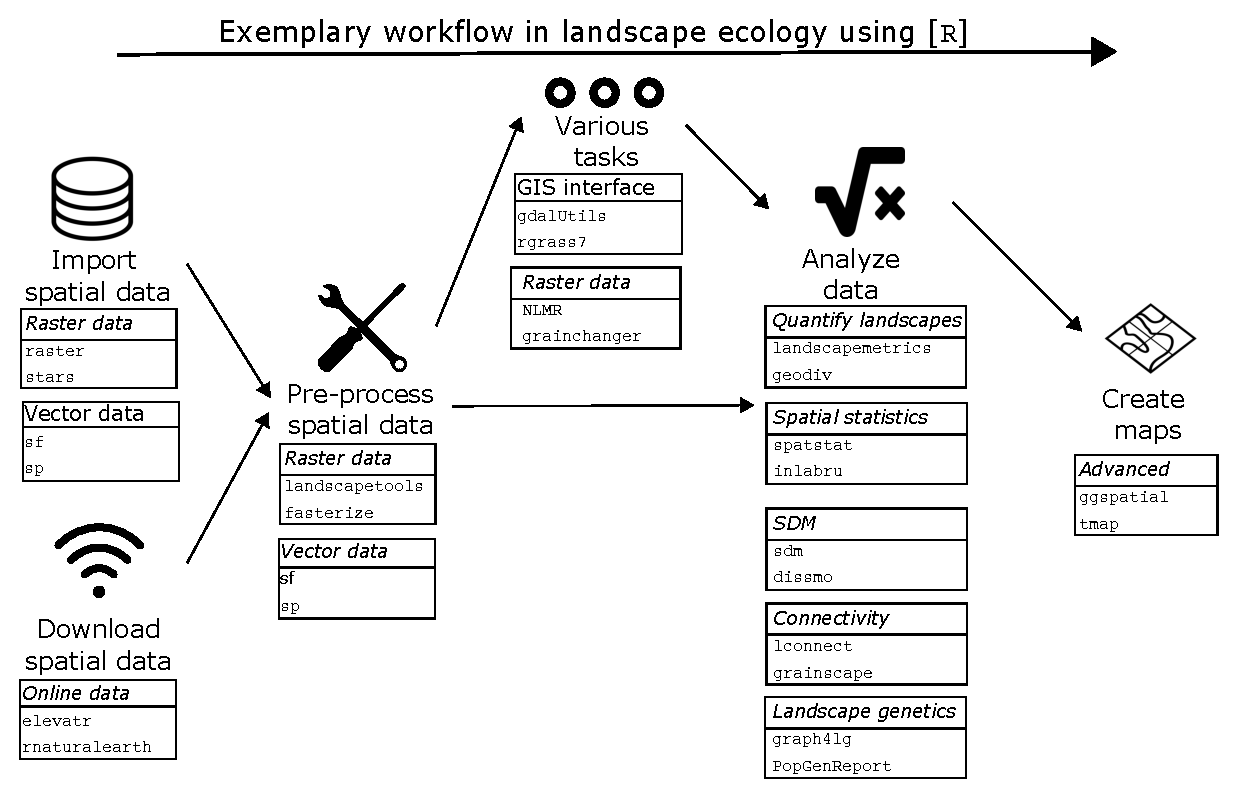
\includegraphics[width=\linewidth]{data/Figure_1} \caption{Exemplary workflow of spatial data analyses for landscape ecology using the \textit{R} programming language. For all major tasks, some example \textit{R} packages are listed. For more packages related to the specific task, see Table \ref{tab:packages}.}\label{fig:fig-workflow}
\end{figure}

\hypertarget{sec:spatrep}{%
\subsection{Spatial data representations}\label{sec:spatrep}}

While base \textit{R} has several built-in data structures, including vectors, matrices, data frames, and lists, yet it has no internal support for reading, processing, or visualizing spatial data.
However, as discussed previously, one strength and core idea of the \textit{R} programming language are its expandability by packages.
Because there is a substantial interest in spatial data analysis, support for spatial data is now provided by many \textit{R} packages (\cite{Lovelace2019}, Table \ref{tab:packages}).
Most spatial data belong to one of two data models, namely spatial raster and spatial vector model, and both data models have several implementations in the \textit{R} language.
Importantly, main \textit{R} packages for spatial data use the external \textit{GDAL} \cite{GDAL/OGRcontributors2020} and \textit{PROJ} \cite{PROJcontributors2021} libraries, which allow for reading and writing of hundreds of spatial data formats, and for coordinates transformation.
Additionally, \textit{R} allows for conversion between data models and specific implementations, which can be useful if given methods only exist for a particular data model or implementation.

In the raster data model, surfaces are divided into cells, where each cell stores a numeric value.
The values could represent discrete phenomena, such as a class number of a land cover category, or continuous phenomena, such as elevation values.
Currently, the most prominent package allowing for raster data representation is \textit{raster} \cite{Hijmans2019}.
A \textit{raster} successor, \textit{terra}, aimed at the simpler interface and improved performance is being developed \cite{Hijmans2021}, however, it could take several years for this package to be adopted by other developers and users.
Alternatively, the \textit{stars} package can be used to read and process raster data focusing on spatial-temporal data cubes \cite{Pebesma2019}.
Additionally, there are packages that improve some basic raster operations in terms of computational performance or compatibility between raster and vector operations, such as \textit{fasterize} \cite{Ross2020}, \textit{rasterDT} \cite{OBrien2020}, or \textit{exactextractr} \cite{Baston2020}.

The vector data model consists of two main elements i) geometries (such as points, lines, polygons) and ii) attributes, where each geometry is connected to a row in the attribute table.
In many cases, this data model allows a more realistic representation of landscape features, however, with higher computational cost \cite{Lovelace2019}.
The \textit{sp} package was the standard for vector data representation for more than ten years \cite{Pebesma2005,Bivand2013}.
As of 2020, more than 500 \textit{R} packages directly depend on or import \textit{sp}.
However, \textit{sp} is not actively developed anymore, and its recommended successor is the \textit{sf} package \cite{Pebesma2018}.
Besides many advantages and strengths of the \textit{sf} package in terms of spatial data handling, it also integrates into the widely used \textit{tidyverse} packages \cite{Wickham2019}.
The \textit{tidyverse} is a collection of \textit{R} packages developed for almost all major tasks of any data analysis project.
Because all \textit{tidyverse} packages follow the same philosophy how to structure data, one strength of the \textit{tidyverse} is its high consistency of usage across its packages \cite{Wickham2019}.
\textit{sf} builds on the idea of ``simple features,'' a standard used to describe spatial geometries using points, lines (two connected points) and polygons (several connected points), and attributes connected to these geometries \cite{Pebesma2019a}.

\hypertarget{spatial-data-download}{%
\subsection{Spatial data download}\label{spatial-data-download}}

Nowadays, spatial data at various scales is available from many online-accessible sources.
A lot of this data are publicly available, either as a direct download or through an API connection, and several packages can use this to download the spatial data directly into an \textit{R} session.
Since publicly available data is becoming more prominent, so are \textit{R} packages to access them.
Packages include \textit{rnaturalearth} \cite{South2017} to access the Natural Earth database to download region and country data, the \textit{elevatr} package to access raster elevation data \cite{Hollister2020}, the \textit{rgbif} package to access the Global Biodiversity Information Facility (GBIF) portal \cite{Chamberlain2017}, the \textit{BIEN} package \cite{Maitner2020} to access the Botanical Information and Ecology Network Database, the \textit{marmap} to download bathymetry data from the ETOPO1 database \cite{Pante2013}, or the \textit{FedData} package \cite{Bocinsky2019} to access the National Land Cover Database (NLCD) data for the USA.
Furthermore, the \textit{getlandsat} package \cite{Chamberlain2018} allows users to download Landsat 8 satellite data, the \textit{MODIS} package \cite{Mattiuzzi2020} to download MODIS products, and \textit{sen2r} \cite{Ranghetti2020} to download Sentinel-2 optical images.
Also, the \texttt{getData()} function from the \textit{raster} package allows users to download climatic and bioclimatic data from WorldClim v1.4.
Additionally, the \textit{rgee} package \cite{Aybar2020} gives access to an extensive catalog of data from Google Earth Engine, including climate data, land cover maps, and satellite imagery.

\hypertarget{spatial-data-processing}{%
\subsection{Spatial data processing}\label{spatial-data-processing}}

Coordinate reference systems (CRS) describe how spatial data is projected from the earth's three-dimensional surface to a two-dimensional surface as required for spatial analysis or creating maps \cite{Lovelace2019,Pebesma2019a}.
This is also referred to as spatial projection and is often the first barrier in spatial data analysis.
It is not only required to have all of the used data in the same projection, but also to select a proper CRS.
This is of importance because the projection into a two-dimensional surface unavoidable leads to distortion, and different CRS are optimized for different properties, regions of the world, and scales \cite{Bivand2013,Lovelace2019}.
Coordinates in spatial data represent one of many coordinate reference systems.
Two main groups of CRS, namely geographical and projected, exist, with each having many members.
Using geographical CRS, positions are specified by latitude and longitude coordinates in degrees.
However, most landscape ecology studies should utilize projected CRSs, which use some measurement units (e.g., meters).
The selection of projected CRS should be based on the property of spatial data that needs to be kept intact (e.g., no distortion of areas, shapes, distances, or angles) and be appropriate for a given study area.
A common way to refer to different CRS is to used codes developed by the European Petrol Survey Group (EPSG).
Tools to find an appropriate CRS for a certain region can be found at \url{https://spatialreference.org}, \url{https://epsg.org}, or \url{http://epsg.io}.
All packages from Section \ref{sec:spatrep} have interfaces for coordinates transformations, allowing unification of spatial projections when the used data have different CRS.

Until 2020, spatial \textit{R} objects stored information about their CRS using Proj4 string representations, and these strings could also be used for CRS transformations.
However, the major changes in upstream software, namely PROJ6 and GDAL3, limited the capabilities of the Proj4 strings and switched to use a new representation called WKT2-2019 for storing the CRS.
Thus, spatial objects saved with degraded Proj4 string representation to \textit{R} file formats could be incorrectly read, and special attention should be given to check their correctness.
Proj4 string representation is also not recommended to set or transform CRS and instead the previously introduced EPSG codes should be used.
A more detailed explanation of the recent CRS changes can be found in \cite{Bivand2020}.

Another common spatial data processing task is required when the available data extends over a larger area than the study region.
In this case, the pre-processing of spatial data should include vector clipping or raster cropping.
Related to that, masking certain areas of the study region using spatial filters (e.g., water bodies, urban areas) can be required.
Packages from Section \ref{sec:spatrep} also allow for these operations.
Additionally, they offer many other operations, such as merging or joining spatial data, extracting values from one dataset into another, raster resolution changes, or vector data simplifications.
A comprehensive collection of methods to aggregate raster values to a coarser resolution can also be found in the \textit{grainchanger} package \cite{Graham2019}.
Furthermore, \textit{landscapetools} is a collection of various utility functions for the raster data model \cite{Sciaini2018}.

Finally, there are several tools for landscape ecology implemented in GIS software, such as \texttt{r.li} or \texttt{r.pi} for GRASS GIS \cite{Wegmann2018,Neteler2012,Porta2017}, terrain analysis methods in SAGA GIS \cite{Conrad2015}, or morphological operations for Google Earth Engine.
It is possible to control several GIS software directly from \textit{R} using dedicated packages, such as \textit{rgrass7} \cite{Bivand2021} for GRASS GIS, \textit{RSAGA} \cite{Brenning2018} for SAGA GIS, and \textit{rgee} \cite{Aybar2020} for Google Earth Engine.
Direct access to these GIS software within \textit{R} allows to create reproducible and sharable \textit{R} scripts, even if functionality is currently not available in \textit{R}.

\begin{table}

\small

\begin{tabularx}{1\textwidth}{|X|}

\hline
\multicolumn{1}{|c|}{\textbf{Box 1: Where to start}} \\

\\

\textbf{1.} Get familiar with basics of \textit{R} programming language. 
Good resources can be found at \url{https://cran.r-project.org/manuals.html}. \\

\textbf{2.} Understand the fundamental spatial data types, i.e., raster data and vector data.
This also includes being able to process the data using the corresponding packages such as \textit{raster} or \textit{sf}. 
These packages also have excellent documentation at \url{https://rspatial.org/raster} and \url{https://r-spatial.github.io/sf}, respectively. \\

\textbf{3.} Be able to transform coordinate reference systems of data from different sources. Depending on the data type, \textit{raster} or \textit{sf} and the corresponding documentations are good starting points. \\

\textbf{4.} Do a quick visualization of the data for inspection or a first glance at the data. 
This can be done with base \textit{R} or -- if already familiar -- \textit{ggplot2}. \\

\textbf{5.} Find suitable \textit{R} package for research questions. 
This can be difficult since research questions, available data and packages are diverse. 
Good starting points are the CRAN Task Views (mainly \url{https://cran.r-project.org/web/views/Spatial.html}) or review papers similar to this one. 
If several packages exist, try all of them and see which ones suites the question and data the best. \\

\textbf{6.} Create publication-quality figures and maps using, e.g., \textit{ggspatial} or \textit{tmap}. 
Help for both packages can be found on the corresponding homepages \url{https://paleolimbot.github.io/ggspatial/index.html} or \url{https://mtennekes.github.io/tmap}. \\

\textbf{7.} Make reproducible \textit{R} scripts publicly available if possible. \\

\textbf{8.} Further excellent resources with applied help about spatial data in \textit{R} can be found \url{https://geocompr.robinlovelace.net}, \url{https://rspatial.org}, or \url{https://r-spatial.org/book/}. \\

\hline
\end{tabularx}
\end{table}

\hypertarget{creating-maps}{%
\subsection{Creating maps}\label{creating-maps}}

Creating maps is essential when working with spatial data.
Maps play an important role in checking the spatial and value-related quality of data, data exploration, and finally communicating results.
\textit{R} allows two major types of maps.
Firstly, static maps in which the developer has full control over the presentation of the map and secondly, interactive maps in which the user can modify the map by, e.g., changing the displayed values.
All packages listed in Section \ref{sec:spatrep} have build-in methods for plotting spatial data using the generic \texttt{plot()} function (Fig. \ref{fig:fig-map}a).
However, the generic functions are focused on quick visual inspection of the data (Fig. \ref{fig:fig-map}a), rather than the creating complete maps as they do not directly support additional map elements (e.g., scale bar, north arrow) nor small multiples maps.

The popular plotting package \textit{ggplot2} (Fig. \ref{fig:fig-map}b) can also visualize spatial data and is build on a layered grammar of graphics, which allows to create maps by combining individual graphical elements (e.g., raster and vector elements) \cite{Wickham2016}.
Additionally, there is an extension especially designed to plot spatial data named \textit{ggspatial}, which provides additional map elements \cite{Dunnington2020}.
For more information about \textit{ggplot2} in general, see \cite{Wickham2016}.
The \textit{tmap} package provides a provides a coherent plotting system intended for drawing maps (Fig. \ref{fig:fig-map}c) \cite{Tennekes2018}.
This package operates in two modes, static and interactive, which means that the same code can be used to create static or interactive maps.
Quick interactive visualization of spatial data can be done with the \textit{mapview} package\cite{Appelhans2020}.
Both, \textit{tmap} and \textit{mapview} build upon the \textit{leaflet} package and leaflet javascript library \cite{Cheng2021}.
Static thematic maps, including proportional symbols, choropleth, or typology maps, can be created with the \textit{cartography} package \cite{Giraud2016}.
Further plotting methods for raster objects can be found in the \textit{rasterVis} package \cite{Lamigueiro2020}.
A slightly different approach to visualizing spatial data is adapted by the \textit{rayshader} package \cite{Morgen-Wall2020} that creates topographic 2D and 3D maps.



\begin{figure}
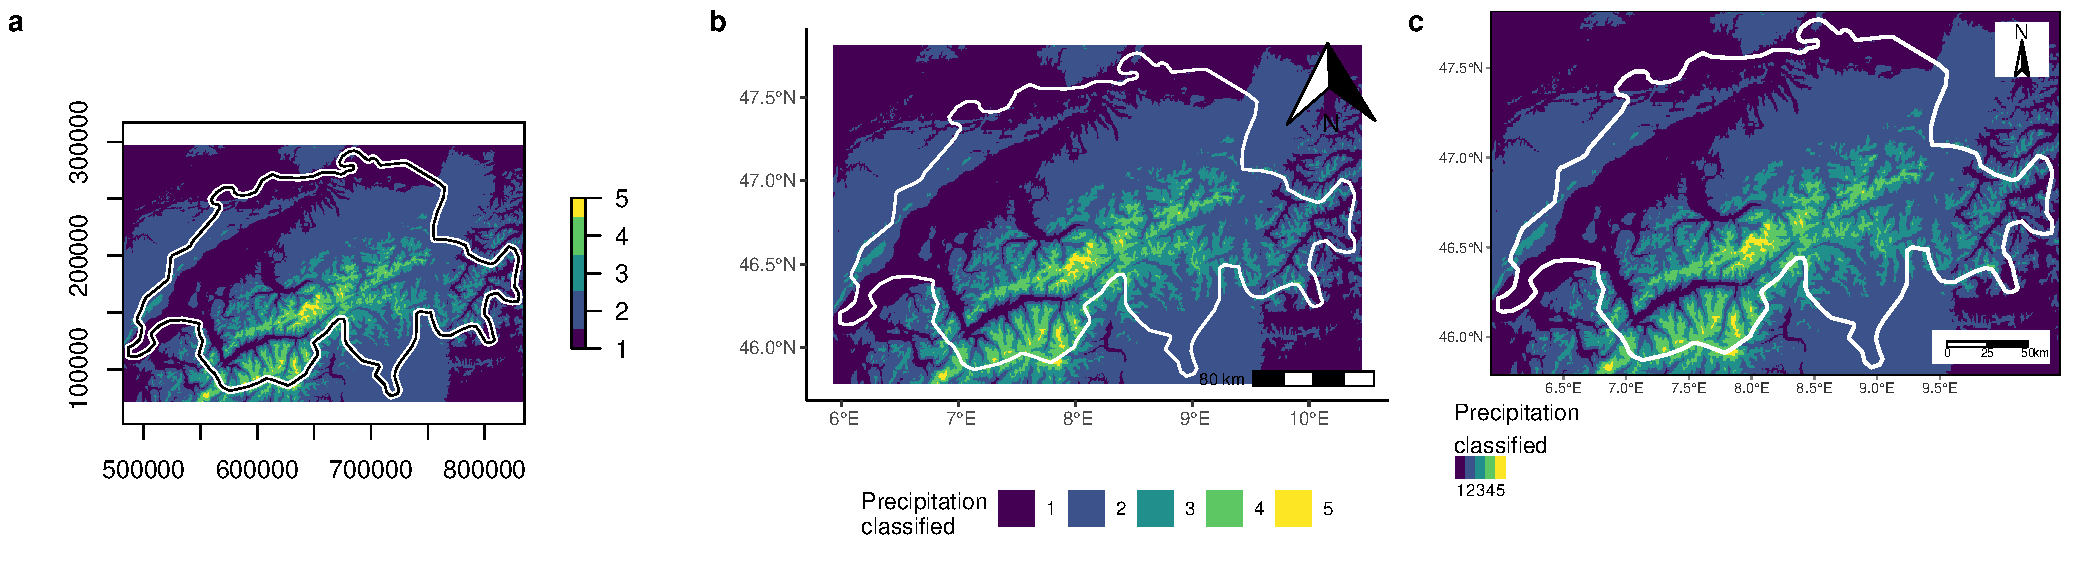
\includegraphics[width=\linewidth]{data/Figure_2} \caption{Comparison of different options to create maps of the total annual precipitation in Switzerland using a) base plot, b) \textit{ggplot2} package, and c) \textit{tmap} package. All three approaches result in similar-looking outputs, but their syntax and capabilities differ. All maps show the total annual precipitation of Switzerland. Data were downloaded with the \textit{raster} package (precipitation data) and \textit{rnaturalearth} package (country borders) package. The code to create the maps can be found in the Appendix.}\label{fig:fig-map}
\end{figure}

\FloatBarrier

\hypertarget{sec:ecological_analysis}{%
\subsection{Ecological analysis}\label{sec:ecological_analysis}}

\hypertarget{sec:landscape_metrics}{%
\paragraph{Quantify landscape characteristics}\label{sec:landscape_metrics}}

One of the most fundamental steps of landscape ecology analyses is to describe and quantify landscape characteristics \cite{Turner2005,Lausch2015}.
For discrete land cover classes, the composition (number and abundance) and configuration (spatial arrangement) of the landscape are often described using landscape metrics \cite{Gustafson1998,Uuemaa2009,Uuemaa2013,Gustafson2019}.
These metrics allow the comparison of different landscapes, quantification of temporal and spatial landscape changes and investigation of interactions between landscape characteristics and ecological processes \cite{Uuemaa2009}.

The introduction of \textit{FRAGSTATS} in 1995 heavily facilitated the use of landscape metrics software \cite{McGarigal2012,Kupfer2012,Gustafson2019} and the \textit{landscapemetrics} package \cite{Hesselbarth2019} allows to calculate the most widely used landscape metrics within the \textit{R} environment.

More recently, surface metrics were suggested as an alternative to landscape metrics for continuous raster data \cite{McGarigal2009}.
The \textit{geodiv} package \cite{Smith2020} allows calculation of gradient surface metrics to facilitate continuous analysis of landscape features.
Additionally, the \textit{belg} package allows calculation of the Boltzmann entropy of a landscape gradient \cite{Nowosad2020}.

Most landscape metrics are represented by a single number depicting specific characteristics of a local landscape.
Another possibility is to derive spatial signatures - a multi-value representation of landscape composition and configuration, such as a co-occurrence histogram \cite{Nowosad2021}.
Spatial signatures calculated for many landscapes can be compared using one of a set of existing distance measures (e.g., Euclidian, Jensen-Shannon, Jaccard).
This enables several types of spatial analysis on categorical raster data, such as searching for similar landscapes, detecting changes between landscape patterns, and spatial clustering of landscapes based on their composition and configuration.
All of the spatial signatures methods mentioned above are implemented in the \textit{motif} package \cite{Nowosad2021}.

\hypertarget{spatial-statistics}{%
\paragraph{Spatial statistics}\label{spatial-statistics}}

Spatial statistics are complimentary to landscape metrics, and can be used to analyze patterns in continuous data (e.g., normalized difference vegetation index, disturbance intensity, topography).
In landscape ecology, spatial statistics has three key uses: i) detecting and correcting for spatial autocorrelation; ii) quantifying and comparing landscape patterns; iii) interpolating data.

Point pattern analysis uses event-level data, such as locations of individuals, and links the spatial pattern to the ecological process.
The \textit{spatstat} package \cite{Baddeley2005} contains functionality for point pattern analysis, including exploratory analysis; simulation of point process models; and modeling fitting, inference, and diagnostics.
A comprehensive textbook covering both theoretical background as well as applied examples can be found here \cite{Baddeley2015}.

Distance-based methods allow for the detection and correction of spatial autocorrelation in data.
It is key to do so as landscape data are highly spatially autocorrelated, and this non-independence can affect inferences from statistical modeling.
The \textit{spdep} package \cite{Bivand2013} has methods for quantifying multiple metrics of spatial autocorrelation and correcting these in a spatial autoregressive model.
The \textit{rinla} \cite{Rue2009} (\url{https://www.r-inla.org}) and \textit{inlabru} \cite{Bachl2019} packages also provide functionality for modeling of spatially structured data.

Finally, the spatial structure of continuous landscapes can be quantified and compared with geostatistical tools, such as variograms and correlograms.
\textit{R} packages \textit{geoR} \cite{Diggle2007} and \textit{gstat} \cite{Pebesma2004} provide functionality for this type of analysis, as well as interpolation methods, known as (co-)kriging.
Geostatistics also allows for spatial data simulations.

\hypertarget{sec:SDM}{%
\paragraph{Species distribution modeling}\label{sec:SDM}}

Species distribution modeling (SDM) examines how landscape patterns (e.g., habitat suitability or resources availability) influence and determine the patterns of species' distributions, mainly to infer ecological processes and predict future species' distributions \cite{Wiersma2011}.
Originated in the 1970s, SDM has experienced numerous methodological advancement, and a large body of literature exists today \cite{Zimmermann2010,Norberg2019}.
Additionally, textbooks introducing basic concepts of SDM in \textit{R} exist \cite{Guisan2017,Fletcher2018}.

Because the used modeling approaches are diverse \cite{Hooten2011,Kerr2011,Fletcher2018}, there is also a large number of \textit{R} packages used for SDMs.
Popular approaches and packages include generalized linear models using, e.g., the \textit{stats} \cite{RCoreTeam2019} package; generalized additive models using, e.g., the \textit{mgcv} \cite{Wood2017} or \textit{lme4} \cite{Bates2015} package; classification and regression trees (CART) using, e.g., the \textit{rpart} \cite{Therneau2019}, \textit{randomForest} \cite{Liaw2002} or \textit{ranger} \cite{Wright2017} package or multivariate data analysis using , e.g., the \textit{ade4} \cite{Dray2007} or \textit{vegan} \cite{Oksanen2019} package.
Also, packages specifically designed for SDM exist, including the \textit{dismo} \cite{Hijmans2017}, \textit{sdm} \cite{Naimi2016}, \textit{ecospat} \cite{Broennimann2020}, \textit{biomod2} \cite{Thuiller2020}, \textit{PresenceAbsence} \cite{Freeman2008}, or \textit{zoon} \cite{Golding2018} packages.
Additionally, packages such as \textit{ENMeval} \cite{Muscarella2014} provide functionality for model tuning and evaluation.

Related to SDMs, there is a growing number of \textit{R} packages to analyze data from tracked animals, to study their movement characteristics, space use, and interaction with other animals and the environment.
These analyses often use results of landscape ecological analyses as predictor variables to explain variation in space use \cite{Signer2015}, behavioral states \cite{Langrock2012}, or habitat selection \cite{Fieberg2020}.
Widely used \textit{R} packages include \textit{ctmm} \cite{Calabrese2016} and \textit{adehabitatHR} \cite{Calenge2006} for home-range estimation, \textit{moveHMM} \cite{Michelot2016} for the classification of behavioral states, and \textit{amt} \cite{Signer2019} for habitat selection.
A recent and very comprehensive overview of \textit{R} packages for the analysis of animal movement data is given by \cite{Joo2020}.

\hypertarget{sec:connectivity}{%
\paragraph{Connectivity}\label{sec:connectivity}}

Connectivity is one of the core elements of landscape structure \cite{Taylor1993} and thus one of the core concepts of landscape ecology \cite{With2019}.
Landscape connectivity describes how landscape characteristics facilitate or hinder the movement of species \cite{Tischendorf2000} or other aspects of mobility, such as dispersal, gene or nutrient flow \cite{With2019}.
While structural connectivity focuses only on landscape characteristics (e.g., movement corridors, barriers), functional connectivity also includes behavior characteristics of the species such as habitat associations and dispersal distances \cite{Tischendorf2000,With2019}.
Given its broad concept, many different measures of connectivity exist \cite{Kindlmann2008}.
At the patch level, structural connectivity can be measured using nearest-neighbor distances or characterizations of the patch neighborhood (e.g., amount of suitable habitat) \cite{Kindlmann2008,With2019}.
Such measures are provided within the \textit{landscapemetrics} package (see \ref{sec:landscape_metrics}).
Furthermore, the \textit{lconnect} package \cite{Mestre2019} and \textit{Makurhini} package \cite{Godinez-Gomez2020} provide several landscape connectivity metrics.
Another way to describe connectivity is based on graph theory with the advantage that functional connectivity can also be included \cite{Kindlmann2008}.
In graph theory \cite{Laita2011}, landscapes are described by nodes (i.e., habitat patches) connected by and functional connections called links (or edges) \cite{Laita2011}.
The \textit{grainscape} package \cite{Chubaty2020} provides a tool to model connectivity based on spatially explicit networks.
More generally, the \textit{igraph} package \cite{Csardi2006} provides functionality for graph theoretic analyses.
Resistance surfaces and least-cost paths are other tools to model functional connectivity which include attributes of the matrix.
The resistance surface describes the effects of facilitating or hindering the landscape's characteristics for an organism moving within it \cite{Adriaensen2003}.
Least-cost paths can be calculated using the \textit{gdistance} package \cite{vanEtten2017}.
Absorbing Markov chains quantify landscape connectivity as the combination of movement and mortality based on the landscape characteristics \cite{Fletcher2019}, and is provided by the recently published \textit{samc} package \cite{Marx2020}.

\hypertarget{sec:landscape_genetics}{%
\paragraph{Landscape genetics}\label{sec:landscape_genetics}}

Landscape genetics investigates how characteristics of landscapes interact with gene flow, genetic drift, and selection \cite{Manel2003}.
Such insights improve our understanding of metapopulation dynamics, speciation, species' distributions, and conservation \cite{Storfer2007}.
By explicitly including landscape characteristics, landscape genetics provides a more detailed analysis than more abstract concepts (e.g., metapopulation genetics) \cite{Holderegger2006}.
As a result of its interdisciplinarity, landscape genetics draws together methods from multiple fields, including landscape ecology, spatial statistics, geography, and population genetics \cite{Storfer2007}.

Since describing connectivity between two locations is one of the fundamental steps of landscape genetics, all packages useful for connectivity (see \ref{sec:connectivity}) are also important for landscape genetics.
Further functionality for landscape genetics such as quantifying and analysing population genetic structure, and hierarchical decomposition analysis can be found in the \textit{graphs4lg} \cite{Savary2020}, \textit{PopGenReport} \cite{Adamack2014,Gruber2015}, \textit{HierDpart} packages \cite{Qin2019}, or \textit{GeNetIt} \cite{Murphy2010}.

\hypertarget{sec:NLM}{%
\paragraph{Neutral landscape models}\label{sec:NLM}}

Neutral landscape models are used to create structured landscapes in the absence of specific ecological and landscape processes as null models against which hypotheses including specific ecological and landscape processes can be tested statistically \cite{Gardner1987,With1997}.
Because neutral landscape models are not based on ecological and landscape processes, many different generic algorithms to create landscapes can be found across several \textit{R} packages.
A comprehensive collection of algorithms to simulate neutral landscape models specifically designed for landscape ecology can be found in the \textit{NLMR} package \cite{Sciaini2018}.
Furthermore, the \textit{RandomFields} package \cite{Schlather2015} allows to simulate Gaussian fields, which could be used as neutral landscape models.

\begin{table}

\scriptsize 

\captionsetup{font=scriptsize}

\caption{Overview of commonly used \textit{R} packages for spatial data and landscape ecology. Packages are sorted by their major application task. The table only includes packages specifically designed for spatial data or landscape ecology.}

\begin{tabularx}{1.35\linewidth}{lrXr}

\hline
Task & \textit{R} package & Describtion & Reference \\
\hline
\multirow{8}{*}{Spatial data} & raster & Raster data handling and analysis & \cite{Hijmans2019} \\
& terra & Raster (and some vector) data handling and analysis & \cite{Hijmans2021} \\
& stars & Spatiotemporal raster data handling and analysis & \cite{Pebesma2019} \\
& fasterize & Polygon to raster conversion & \cite{Ross2020} \\
& rasterDT & Faster alternatives for some raster functions & \cite{OBrien2020} \\
& exactextractr & Summarize raster values over polygonal areas & \cite{Baston2020} \\
& sp & Vector data handling and analysis & \cite{Pebesma2005,Bivand2013} \\
& sf & Vector data handling and analysis & \cite{Pebesma2018} \\
\hline
\multirow{6}{*}{Spatial data download} & rnaturalearth & Download region and country data & \cite{South2017} \\
& elevatr & Download elevation data & \cite{Hollister2020} \\
& rgbif & Download biodiversity data & \cite{Chamberlain2017} \\
& BIEN & Download plant diversity, function and distribution data & \cite{Maitner2020} \\
& marmap & Download and manipulate bathymetric data & \cite{Pante2013} \\
& FedData & Download geospatial data from US federal sources & \cite{Bocinsky2019} \\
& getlandsat & Download satellite data from Landsat 8 & \cite{Chamberlain2018} \\
& MODIS & Download satellite data from MODIS & \cite{Mattiuzzi2020} \\
& sen2r & Download satellite data from Sentinel & \cite{Ranghetti2020} \\
\hline
\multirow{3}{*}{Interfacing to GIS} & rgrass7 & Interface between GRASS7 and R  & \cite{Bivand2021} \\
& RSAGA & Interface between SAGA and R & \cite{Brenning2018} \\
& rgee &  Download data from Google Earth Engine & \cite{Aybar2020} \\
\hline
\multirow{7}{*}{Creating maps} & rasterVis & Vizualuzation of raster data & \cite{Lamigueiro2020} \\
& ggspatial & Spatial extension for ggplot2 & \cite{Dunnington2020} \\
& cartography & Create cartographic maps & \cite{Giraud2016} \\
& tmap & Create thematic maps & \cite{Tennekes2018} \\
& mapview & Interactive viewing of spatial data & \cite{Appelhans2020} \\
& leaflet & Create interactive web maps & \cite{Cheng2021} \\
& rayshader & Create 2D and 3D data visualizations & \cite{Morgen-Wall2020} \\
\hline
\multirow{4}{*}{\shortstack[l]{Quantifying landscape\\characteristics}} & landscapemetrics & Quantify categorical landscape patterns & \cite{Hesselbarth2019} \\
& belg & Calculate the Boltzmann entropy & \cite{Nowosad2020} \\
& motif & Pattern-based spatial analysis & \cite{Nowosad2021} \\
& geodiv & Quantify continuous landscape patterns & \cite{Smith2020} \\
\hline
\multirow{6}{*}{\shortstack[l]{Spatial statistics}} & spatstat & Point pattern analysis & \cite{Baddeley2005} \\
& spdep & Quantify and correct for spatial autocorrelation & \cite{Bivand2013} \\
& rinla & Fitting Bayesian spatio-temporal models using INLA & \cite{Rue2009} \\
& inlabru & Fitting Bayesian spatio-temporal models using INLA & \cite{Bachl2019} \\
& geoR & Variograms, correlograms and (co-)kriging & \cite{Diggle2007} \\
& gstat & Variograms, correlograms and (co-)kriging & \cite{Pebesma2004} \\
\hline
\multirow{8}{*}{\shortstack[l]{Species distribution\\modeling}} & dismo & Methods for species distribution modeling & \cite{Hijmans2017} \\
& sdm & Species distribution models using individual and community-based approaches & \cite{Naimi2016} \\
& ecospat & Species distribution, niche quantification and community assembly & \cite{Broennimann2020} \\
& biomod2 & Species distribution modeling, ensemble of models and ensemble forecasting & \cite{Thuiller2020} \\
& PresenceAbsence & Evaluating of presence-absence models & \cite{Freeman2008} \\
& zoon & Reproducible and remixable species distribution modelling & \cite{Golding2018} \\
& ENMeval & Model tuning and evaluation & \cite{Muscarella2014} \\
& adehabitatHR, adehabitatHS & Home range and habitat selection modelling & \cite{Calenge2006} \\
& amt & Manage and analyze animal movement data &\cite{Signer2019} \\
& ctmm & Fit continuous time movement models &\cite{Calabrese2016} \\
& moveHMM & Fit hidden Markov models to movement data &\cite{Michelot2016} \\
\hline
\multirow{5}{*}{Connectivity} & lconnect & Calculate landscape connectivity metrics & \cite{Mestre2019} \\
& Makurhini & Calculate fragmentation and landscape connectivity indices & \cite{Godinez-Gomez2020} \\
& grainscape & Calculate minimum planar graph and grains of connectivity models & \cite{Chubaty2020} \\
& gdistance & Distances and routes on geographical grids & \cite{vanEtten2017} \\
& samc & Functions for working with absorbing Markov chains & \cite{Marx2020} \\
\hline
\multirow{4}{*}{Landscape genetics} & graph4lg & Build graphs for landscape genetics analysis & \cite{Savary2020} \\
& PopGenReport & Framework to analyse population genetic data & \cite{Adamack2014,Gruber2015} \\
& HierDpart & Calculating and decomposing hierarchical diversity metrics & \cite{Qin2019} \\
& GeNetIt & Spatial graph-theoretic genetic gravity models & \cite{Murphy2010} \\
\hline
\multirow{4}{*}{various} & NLMR & Simulate neutral landscape models & \cite{Sciaini2018} \\
& RandomFields & Simulation and analysis of random fields & \cite{Schlather2015} \\
& landscapetools & Utility functions for raster data & \cite{Sciaini2018}  \\
& grainchanger & Data aggregation methods for raster data & \cite{Graham2019} \\
\hline

\end{tabularx}

\label{tab:packages}

\end{table}

\FloatBarrier

\hypertarget{survey-of-usage-by-landscape-ecology-community}{%
\section{\texorpdfstring{Survey of \textit{R} usage by landscape ecology community}{Survey of  usage by landscape ecology community}}\label{survey-of-usage-by-landscape-ecology-community}}

To better understand how the landscape ecology community uses \textit{R}, we conducted a short survey using mailing lists and social media to reach the community.
Thus, the survey was not necessarily representative for all skill levels of \textit{R} users and results are most likely biased towards more advanced users.
Also, the survey did not include any personal questions, such as age or country of residence, which might affect the representation of the survey.
All raw data and scripts to analyze the data can be found at \url{https://github.com/r-spatialecology/Hesselbarth_et_al_CLER}.

In total, the survey was answered by 109 participants, of which the majority were either ``PhD students'' (33\%), followed by ``Post-Docs'' (26.6\%) and ``Professors'' (14.7\%).
Other, less frequent answers were ``Data scientists,'' ``None of the above,'' ``Government employees,'' ``Master's degree student'' and ``Bachelor's degree student'' (in decreasing order).

Most people use \textit{R} either ``daily'' (53.2\%) or a ``few times a week'' (36.7\%).
Almost half of all participants described themselves as ``advanced'' users (46.8\%), while 40.4\% described themselves as ``intermediate'' users.
Related to this, about half of the participants either implemented their own package (21.1\%) or plan to do so in the future (22\%) and most of these packages are hosted on \textit{GitHub} and/or \textit{CRAN}.

We asked the participants to select which terms describe their research topics the best, and options that were selected by more than 10\% of participants included ``biodiversity,'' followed by ``land use management,'' ``landscape connectivity,'' and ``nature conservation'' (Fig. \ref{fig:fig-survey}a).

Next, we were interested in the most important tasks to the workflow of the participants.
Not surprisingly, ``(pre-)processing of data,'' ``spatial statistics,'' and ``creating maps'' were the most selected options (Fig. \ref{fig:fig-survey}b).
The available options seemed to describe the most important task to the workflow quite well since only very few participants selected the ``others'' option (all options with less than five total answers were classified as ``others'').

More people use the raster data model (72.5\%) in comparison to the vector data model (27.5\%).
This was also represented in the most used \textit{R} packages (Fig. \ref{fig:fig-survey}c).
When asked for the three most used packages, participants of the survey listed 93 packages in total.
The \textit{raster} package was mentioned the most, followed by the \textit{sf} package.
Both packages are designed for basic and advanced data handling and processing of raster and vector data, respectively, representing the results of Fig. \ref{fig:fig-survey}c.
Nevertheless, the large availability and usage of different \textit{R} packages across the community can be seen in the large ``others'' option (packages mentioned by less than 5 participants; 35.9\%).

Lastly, when asked how useful \textit{R} is currently for landscape ecology, the vast majority of participants answered with either ``very useful'' or ``useful'' (summarized 90.8\%) and only very few participants evaluated \textit{R} as ``intermediate,'' ``not useful'' or ``not useful at all'' (summarized 9.2\%; Fig. \ref{fig:fig-survey}d).



\begin{figure}

{\centering 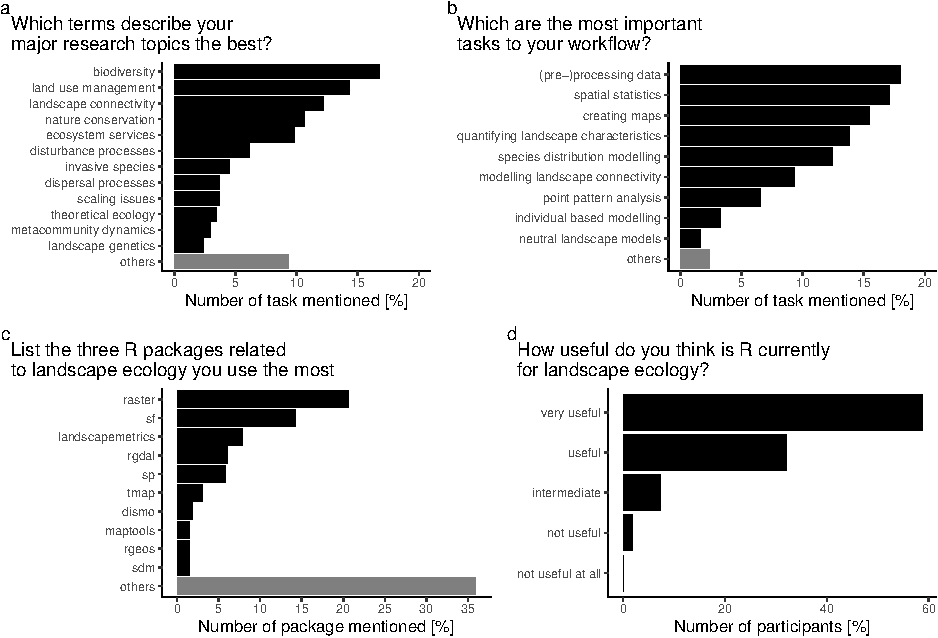
\includegraphics[width=\textwidth]{Manuscript_files/figure-latex/fig-survey-1} 

}

\caption{Results of the online survey about open-source software tools in \textit{R} for landscape ecology. Results include a) which terms describe major research topics the best, b) the most important workflow task, c) the most used \textit{R} packages and d) the overall usefulness or \textit{R} for landscape ecology. The ``others'' category includes all answers with less than five total mentions.}\label{fig:fig-survey}
\end{figure}

The survey also included a section in which participants could list methods and tools currently missing in \textit{R} and answers to this question were very diverse.

Overall, 23.9\% of the participants reported that currently no packages and functionality are missing for them or they lack the overview to answer the question.
There were three most common topics across the answers of the participants.
Firstly, many participants (12.8\%) wished for a better computational performance of \textit{R} in terms of speed and required RAM, especially for larger data sets.
Secondly, participants are missing specific approaches to quantify landscape characteristics (such as surface metrics), or are wishing for an improvement of currently available approaches to quantify landscape characteristics (9.2\%).
Thirdly, many participants (8.3\%) are currently missing advanced and easy-to-apply methods to create high-quality maps or other visualization-related functionality.

\hypertarget{conclusions}{%
\section{Conclusions}\label{conclusions}}

Since its first introduction in 1995, \textit{R} has come a long way from an exclusively statistical programming language to a powerful landscape ecology tool.
Today, many \textit{R} packages, mainly developed by the community itself, provide a vast collection of functions and algorithms aimed at spatial data handling and analysis.
The highly dynamic development of \textit{R} packages for landscape ecology also shows the strength of open-source software with its high innovation, transparency, reliability, and longevity.
However, since landscape ecology constantly develops and improves, consequently also the \textit{R} programming language and its packages are under constant change to adapt to these new developments.

A comprehensive collection of \textit{R} software packages exists to handle the most common tasks of landscape ecology.
Because it is possible to import, modify, analyze, and visualize spatial data all in the same scripted programming environment, \textit{R} allows for transparent and reproducible workflows.
Scripts including all analysis steps and parameter settings can easily be shared, thus the script-based characteristic of the \textit{R} programming language allows to easily distribution and reproduction of analysis across all major operation systems (e.g., Windows, macOS, Linux), as demonstrated by the \textit{R} script in the appendix.
This is a big advantage over point-and-click software interfaces where analysis steps and parameter settings can only be described but not shared, and furthermore, are often only available for certain operating systems.
This also allows users to easily interchange, modify, or adapt methods from other related and unrelated fields.

The survey revealed that the landscape ecology community is overall satisfied with the capabilities of the \textit{R} programming language for landscape ecology.
Furthermore, the survey showed that many members of the landscape ecology community actively develop \textit{R} packages themselves, demonstrating that tools are constantly added and updated.

Landscape ecology combines many different research topics and methodological approaches, and most of them heavily rely on spatial data.
While the \textit{R} programming language is generally well suited to handle, analyze and visualize spatial data, the increasing availability of large data sets also leads to the challenges of increased computational demands, in terms of computational time as well as memory requirements, the \textit{R} programming language has to face.
Some packages discussed herein, such as \textit{raster} and \textit{terra}, already provide solutions by processing data in chunks small enough to be stored in RAM memory.
Furthermore, parallel processing, including the use of high performance clusters, is also provided by several \textit{R} packages.
While this is outside the scope of this manuscript, further resources about parallel processing in \textit{R} can be found here \cite{Bengtsson2020,Schubert2019,McCallum2012}.
Furthermore, as the individual fields collected under the umbrella of landscape ecology develop, so will the need for \textit{R} packages related to those fields.
Nevertheless, as the development of \textit{R} packages over the past years clearly demonstrated, the landscape ecology community is ready to face these challenges.

\FloatBarrier

\hypertarget{acknowledgments}{%
\subsection{Acknowledgments}\label{acknowledgments}}

We are thankful to all members of the `Coastal Ecology and Conservation Lab' at the University of Michigan for comments on an early draft of the manuscript.
We would like to thank two anonymous reviewers for their valuable comments on earlier drafts of the manuscript.

\hypertarget{conflict-of-interest}{%
\paragraph{Conflict of interest}\label{conflict-of-interest}}

MHKH and JN are authors of the \textit{landscapemetrics} and \textit{landscapetools} package.
MHKH is author of the \textit{NLMR} package.
JN is author of \textit{belg} and \textit{motif} package. JS is author of the \textit{amt} package. LJG is author of the \textit{grainchanger} package.

\hypertarget{funding}{%
\paragraph{Funding}\label{funding}}

LJG was supported by the Natural Environment Research Council (NERC) grant \textit{A complex-systems approach to improve understanding of the biodiversity-landscape structure relationship}, grant number NE/T009373/1.
Other authors did not receive any funding for this research.

\hypertarget{availability-of-data-and-material-data-transparency}{%
\paragraph{Availability of data and material (data transparency)}\label{availability-of-data-and-material-data-transparency}}

All raw data and scripts to analyze the data can be found at \url{https://github.com/r-spatialecology/Hesselbarth_et_al_CLER}.

\hypertarget{author-contributions}{%
\paragraph{Author contributions}\label{author-contributions}}

MHKH and JN designed the survey form and analyzed the responses of the participants.
MHKH and JN drafted the manuscript with contributions of JS and LJG and all authors contributed critically to the manuscript and gave final approval for publication.
We used the `sequence--determines--credit' approach (SDC) for the sequence of authors.

\hypertarget{human-and-animal-rights-and-informed-consent}{%
\paragraph{Human and Animal Rights and Informed Consent}\label{human-and-animal-rights-and-informed-consent}}

This article does not contain any studies with human or animal subjects performed by any of the authors.

\hypertarget{important-references}{%
\subsubsection{Important references}\label{important-references}}

\noindent \textbullet \textbullet \cite{Bivand2020}: Recent and comprehensive overview of general developments of \textit{R} to analyze spatial data demonstrating the capabilities of the programming language to analyze spatial data.

\noindent \textbullet \textbullet \cite{Lovelace2019}: Comprehensive textbook about spatial data handling and analyzing including many useful applied code examples.

\noindent \textbullet \cite{Gustafson2019}: This review presents an overview of the developments and the state of the art for quantifying landscape spatial pattern including lessons learned by the author.

\noindent \textbullet \cite{Lai2019}: This review demonstrates that the \textit{R} programming language is widely used in ecology including possible reasons for the wide spread use.


\bibliographystyle{spphys}
\bibliography{bibliography.bib}

\end{document}
